\chapter{General methods}
\label{chap:methods}

\section{Binary number formats}
\label{sec:numbers}

	\subsection{Integers}
	\label{sec:integers}

The simplest way to represent a real number in bits is the integer format. An $n$-bit signed integer starts with a
sign bit followed by a sequence of integer bits, that are decoded as a sum of powers of two with exponents $0,1,...,n-2$.
An positive integer $x$ with signbit $b_0 = 0$ is therefore decoded in bits $b_1,...,b_{n-2}$ as
\begin{equation}
x = \sum_{i=1}^{n-2} 2^{i-1} b_i
\end{equation}
To avoid multiple representations of zero and to simplify hardware implementations, negative integers, with a sign bit (red) being 1,
are decoded with two's complement interpretation (denoted with an underscore) by flipping all other bits and adding $1$ \citep{Choo2003}.
For example in the 4-bit signed integer format (Int4), ${\color{psign}1}110_{\op{Int4}} = {\color{psign}1}010\_ = -2$.
The largest representable integer for a format with $n$ bits is therefore $2^{n-1}-1$ and the spacing between
representable integers is always 1.

	\subsection{Fixed-point numbers}
	\label{sec:fixpoints}

Fixed-point numbers extend the integer format with $n_f$ fraction bits to $n_i$ signed integer bits to decode an additional sum of
powers of two with negative exponents $-1,-2,...,-n_f$. A positive fixed-point number is
\begin{equation}
x = \sum_{i=1}^{n_i-2} 2^{i-1} b_i  + \sum_{i=1}^{n_f} 2^{-i} b_{n_i-2+i}
\label{eq:fixedpoint}
\end{equation}
Every additional fraction bit reduces the number of integer bits, for example Q6.10 is the 16-bit fixed-point format with
6 signed integer bits and 10 fraction bits.

Flexibility regarding the dynamic range can therefore be achieved with integer arithmetic if fixed-point numbers are used
\citep{Russell2017}. Unfortunately, we did not achieve convincing results with integer arithmetic for the applications in this
study, as rescaling of the equations is desired to place many arithmetic calculations near the largest representable number
\citep{Klower2019}. However, any result beyond will lead to disastrous results, as integer overflow usually returns a negative
value following a wrap-around behaviour.

	\subsection{Floating-point numbers}
	\label{sec:floats}

The IEEE standard on floating-point arithmetic defines how floats encode a real number $x$ in terms of a sign, and several
exponent and significant bits
\begin{equation}
x = (-1)^{sign~bit} \cdot 2^{e-bias} \cdot (1+f)
\label{eq:float}
\end{equation}
The exponent bits $e$ are interpreted as unsigned integers, such that $e-bias$ converts them effectively to signed integers.
The significant bits $f_i$ define the significand as $f = \sum_{i=1}^{n_f} f_i 2^{-i}$ such that $(1+f)$ is in the bounds $[1,2)$.
An 8-bit float encodes a real number with a sign bit (red), $n_e = 3$ exponent bits (blue) and $n_f=4$ fraction bits (black) as
illustrated in the following example
\begin{equation}
3.14 \approx {\color{psign}0}{\color{pexpo}100}1001_{\op{Float8}} = (-1)^{\color{psign}0} \cdot 2^{{\color{pexpo}4}-bias}
\cdot (1+2^{-1}+2^{-4}) = 3.125
\label{eq:float_pos}
\end{equation}
with $bias=2^{n_e-1} - 1 = 3$. Exceptions to Eq. \ref{eq:float} occur for subnormal numbers, infinity (Inf) and Not-a-Number
(NaN) when all exponent bits are either zero (subnormals) or one (Inf when f=0, or NaN else). 16-bit half-precision floatin-point 
numbers (Float16) have 5 exponent bits and 10 significant bits. A truncated version of the Float32 format (8 exponent bits, 23 significant bits)
is BFloat16 with 8 exponent bits and 7 significant bits. Characteristics of various formats are summarised in Table \ref{tab:formats}.
A format with more exponent bits has a wider dynamic range of representable numbers but lower precision, as fewer bits are available
for the significant. All floating-point formats have a fixed number of significant bits. Consequently, they have a constant number of
significant digits throughout their range of representable numbers (subnormals excluded), which is in contrast to posit numbers,
which are introduced in the next section.

\begin{table}[htbp]
\center
\begin{tabular}{l | r | r | l | l | r | r}
Format & bits & exp bits & $minpos$ & $maxpos$ & $\epsilon$ &  \% NaR \\
\hline
Float64    & $64$ & $11$ & $5.0 \cdot 10^{-324}$ & $1.8 \cdot 10^{308}$  & $16.3$ & $0.0$ \\
Float32    & $32$ & $8$ & $1.0 \cdot 10^{-45}$ & $3.4 \cdot 10^{38}$ & $7.6$ & $0.4$ \\
Float16    & $16$ & $5$ & $6.0 \cdot 10^{-8}$ & $65504$ & $3.7$ & $3.1$ \\
BFloat16    & $16$ & $8$ & $ 9.2 \cdot 10^{-41}$ & $3.4 \cdot 10^{38}$ & $2.8$ & $0.4$  \\
Float8 & $8$ & $3$ & $1.5 \cdot 10^{-2}$ & $15.5$ & $1.9$ & $12.5$\\
\hline
Posit32    & $32$ & $2$ &  $7.5 \cdot 10^{-37}$ & $7.5 \cdot 10^{37}$ & $8.8$ & $0.0$ \\
Posit(16,1) & $16$ & $1$ & $3.7 \cdot 10^{-9}$ & $3.7 \cdot 10^{9}$ & $4.3$ & $0.0$\\
Posit(16,2) & $16$ & $2$ & $1.4 \cdot 10^{-17}$ & $1.4 \cdot 10^{17}$ & $4.0$ & $0.0$\\
Posit(8,0) & $8$ & $0$ & $1.5 \cdot 10^{-2}$ & $64$ & $2.2$ & $0.4$  \\
\hline
Int16 & $16$ & $0$ & $1$ & $32767$ & $0.8$ & $0$\\
Q6.10 & $16$ & $0$ & $9.8 \cdot 10^{-4}$ & $32.0$ & $3.7$ & $0$\\
\hline
LogFixPoint16 & $16$ & $15$ & $5.4 \cdot 10^{-20}$ & $1.8 \cdot 10^{19}$ & $3.2$ & $0.0$\\
Approx14 & $14$ & $13$ & $5.4 \cdot 10^{-20}$ & $9.1 \cdot 10^{18}$ & $2.6$ & $0.8$
\end{tabular}
\vspace{10pt}
\caption{Some characteristics of various number formats. $minpos$ is the smallest representable positive number,
$maxpos$ the largest. The machine precision $\epsilon$, is the decimal precision at $1$. \% NaR denotes the
percentage of bit patterns that represent not a number (NaN), infinity or not a real (NaR).}
\label{tab:formats}
\end{table}

	\subsection{Logarithmic fixed-point numbers}
	\label{sec:logfixs}

Fixed-point numbers have a limited range and for the applications in this study an unsuitable distribution of decimal precision.
However, logarithmic fixed-point numbers are similar to floating-point numbers. A $n$-bit logarithmic fixed-point number is defined as
\begin{equation}
x = (-1)^{sign~bit} \cdot 2^e
\label{eq:logfixpoint}
\end{equation}
where $e$ is encoded as an $(n-1)$-bit fixed-point number (Eq. \ref{eq:fixedpoint}).
Consequently, logarithmic fixed-point numbers are equally spaced in log-space and
have a perfectly flat decimal precision throughout the dynamic range of representable
numbers (Fig. \ref{fig:decimal_precision}). We call the 16-bit logarithmic fixed-point numbers
with 7 signed integer bits and 8 fraction bits LogFixPoint16. Approx14 is a proprietary number
 format developed by Singular Computing, which is essentially a 14-bit logarithmic fixed-point
 numbers with 7 signed integer bits and 6 fraction bits.

Logarithmic number formats have the advantage that no rounding error is applied for multiplication, as the addition of the exponents
is exact with fixed-point numbers (as long as no under or overflow occurs). Hence, multiplication with LogFixPoint16 and Approx14
is not just exact but also fast, due to implementation as integer addition. Conversely, addition with logarithmic numbers is difficult.
Adding two logarithmic numbers involves the computation of a logarithm, which, however, for low precision numbers can be implemented as a table look-up.

Both LogFixPoint16 and Approx14 come with a round-to-nearest rounding mode in log2-space.  We consider $x_1 = 2^0 = 1$
and $x_2 = 2^1 = 2$ as two representable numbers as an example with $x$ in between. With round-to-nearest (and tie to even)
in linear-space all numbers $x$ larger equal $1.5$ are round up and others round down. With round-to-nearest in log2-space
$2^{\tfrac{1}{2}} = \sqrt{2} = 1.414...$ is the log-midpoint as $\log_2(\sqrt{2}) = 0.5$. Consequently, the numbers between
$\sqrt{2}$ (inclusive) and $2$ will be round up and only numbers between $1$ and less than $\sqrt{2}$ will round down.
Hence, the linear range of numbers that will be round up is larger than those that will round down. This rounding is biased
as the expectation of rounded uniformly distributed values between $1$ and $2$ is not equal to the expectation without rounding.
Let $\op{round}_{\log_2}(x)$ be the round-to-nearest function in log2-space and $x$ be drawn $N$-times from a random uniform
distribution $U(1,2)$, then
\begin{equation}
    \frac{1}{N}\sum_i^N x_i = 1.5 \neq \frac{1}{N}\sum_i^N \op{round}_{\log_2}(x_i) = 3 - \sqrt{2} = 1.586...
    \label{eq:biased_rounding}
\end{equation}
 We will investigate the effect of this round-to-nearest in log2-space in section \ref{sec:mixed}.


	\subsection{Posit numbers}
	\label{sec:posits}

Posit numbers arise from a projection of the real axis onto a circle (Fig. \ref{fig:circle}), with only one bitpattern for zero and one
for Not-a-Real (NaR, or complex infinity), which serves as a replacement for Not-a-Number (NaN). The circle is split into
\emph{regimes}, determined by a constant $useed$, which always marks the north-west on the posit circle (Fig. \ref{fig:circle}b).
Regimes are defined by $useed^{\pm1}$, $useed^{\pm2}$, $useed^{\pm3}$, etc. To encode these regimes into bits, posit
numbers extend floating-point arithmetic by introducing regime bits that are responsible for the dynamic range of representable
numbers. Instead of having a fixed length, regime bits are defined as the sequence of identical bits after the sign bit, which are
eventually terminated by an opposite bit. The flexible length allows the significand (or mantissa) to occupy more bits when less
regime bits are needed, which is the case for numbers around one. A resulting higher precision around one is traded against a
gradually lower precision for large or small numbers. A positive posit number $p$ is decoded as
\citep{Gustafson2017,Gustafson2017a,Klower2019} (negative posit numbers are converted first to their two's complement, see
Eq. \ref{eq:2comp})
\begin{equation}
p = (-1)^{sign~bit} \cdot useed^k \cdot 2^e \cdot (1+f)
\label{eq:posit}
\end{equation}
where $k$ is the number of regime bits. $e$ is the integer represented by the exponent bits and $f$ is the fraction which is
encoded in the fraction (or significant) bits. The base $useed = 2^{2^{e_s}}$ is determined by the number of exponent bits
$e_s$. More exponent bits increase - by increasing $useed$ - the dynamic range of representable numbers for the cost of precision.
The exponent bits themselves do not affect the dynamic range by changing the value of $2^e$ in Eq. \ref{eq:posit}. They fill gaps of
powers of 2 spanned by $useed = 4,16,256,...$ for $e_s=1,2,3,...$, and every posit number can be written as $p = \pm 2^n \cdot (1+f)$
with a given integer $n$ \citep{Gustafson2017,Chen2018}. We will use a notation where Posit($n$,$e_s$) defines the posit numbers
with $n$ bits including $e_s$ exponent bits. A posit example is provided in the Posit(8,1)-system (i.e. $useed = 4$)
\begin{equation}
57 \approx {\color{psign}0}{\color{pregime}111}{\color{pregimet}0}{\color{pexpo}1}11_{\op{Posit}(8,1)} = (-1)^{\color{psign}0}
\cdot 4^{\color{pregime}2} \cdot 2^{\color{pexpo}1} \cdot (1+2^{-1}+2^{-2}) = 56
\label{eq:posit_pos}
\end{equation}
The sign bit is given in red, regime bits in orange, the terminating regime bit in brown, the exponent bit in blue and the fraction bits in black.
The $k$-value is inferred from the number of regime bits, that are counted as negative for the bits being 0, and positive, but subtract 1,
for the bits being 1. The exponent bits are interpreted as unsigned integer and the fraction bits follow the IEEE floating-point standard
for significant bits. For negative numbers, i.e. the sign bit being 1, all other bits are first converted to their two's complement (\cite{Choo2003},
denoted with an underscore subscript) by flipping all bits and adding 1,
\begin{equation}
\begin{split}
-0.28 &  \approx 11011110_{\op{Posit}(8,1)} = {\color{psign}1}{\color{pregime}0}{\color{pregimet}1}{\color{pexpo}0}0010\_ \\
& = (-1)^{\color{psign}1} \cdot 4^{\color{pregime}-1} \cdot 2^{\color{pexpo}0} \cdot (1+2^{-3}) = -0.28125.
\end{split}
\label{eq:2comp}
\end{equation}
After the conversion to the two's complement, the bits are interpreted in the same way as in Eq. \ref{eq:posit_pos}.

Posits also come with a no overflow/no underflow-rounding mode: Where floats overflow and return infinity when the exact result of an
arithmetic operation is larger than the largest representable number ($maxpos$), posit arithmetic returns $maxpos$ instead, and similarly
for underflow where the smallest representable positive number ($minpos$) is returned. This is motivated as rounding to infinity returns a
result that is infinitely less correct than $maxpos$, although often desired to indicate that an overflow occurred in the simulation.
Instead, it is proposed to perform overflow-like checks on the software level to simplify exception handling on hardware \citep{Gustafson2017a}.
Many functions are simplified for posits, as only two exceptions cases have to be handled, zero and NaR. Conversely, Float64 has more than
$10^{15}$ bitpatterns reserved for NaN, but these only make up $< 0.05\%$ of all available bit patterns. The percentage of redundant
bitpatterns for NaN increases for floats with fewer exponent bits (Table \ref{tab:formats}), and only poses a noticeable issue for Float16
and Float8.

The posit number framework also highly recommends \emph{quires}, an additional register on hardware to store intermediate results.
Dot-product operations are fused with quire arithmetic and can therefore be executed with a single rounding error, which is only applied
when converting back to posits. The quire concept could also be applied to floating-point arithmetic (fused multiply-add is available on
some processors), but is technically difficult to implement on hardware for a general dot-product as the required registers would need
to be much larger in size. For fair comparison we do not take quires into account in this study. The posit number format is explained in
more detail in \cite{Gustafson2017a}. In order to use posits on a conventional CPU we developed for the Julia programming language
\citep{Bezanson2017} the posit emulator \emph{SoftPosit.jl} \citep{Klower2019a}, which is a wrapper for the C-based library SoftPosit
\citep{Leong2020}. The type-flexible programming paradigm, facilitated by the Julia language, is outlined in \ref{sec:julia}.

\subsection{Self-organizing numbers}
\label{sec:sonums}

The design of floating-point numbers in the 1970s and 1980s was motivated to meet several criteria: (i) hardware-friendly, i.e. the number format was designed to map easily from existing arithmetic circuits into bits; (ii) multi-purpose, i.e. initially declared as format for \emph{scientific computations} it was supposed to be able to represent very large numbers $O(10^{-100})$ to $O(10^{-300})$ as well as very tiny numbers $O(10^{-100})$ to $O(10^{-300})$ with the same precision, to allow the use in many different fields of science (iii) error analysis-friendly, i.e. especially Float64 was designed to allow for very precise calculations, such that most scientists would not need to perform a numerical error analysis.

In the following we will relax these criteria and seek to find a number format that has the lowest rounding errors for a given application. We thereby ignore any hardware limitations, and create this number format purely on the basis of a software emulator. In fact, we end up designing it based on look-up tables. Arithmetic operations are with look-up tables not functions that calculate the result based on the inputs, but return the result from an array where the inputs determine the indices. This is in general only feasible for a small set of different inputs, as the underlying arrays have to be stored in memory. Look-up tables for 16-bit arithmetic, as considered here, are of a size of several GB which is unfeasible for current computing hardware. Look-up tables therefore are stored in RAM whereas a storage in much smaller low-level caches is necessary for speed. Every additional bit quadruples the size, such that look-up tables are only attractive for very low precision number formats or can be used for software emulators for up to 16 bit. We also do not aim to create a multi-purpose number format, but conversely a number format that is flexible enough to accommodate the precision requirements of a given algorithm as good as possible.

Motivated by the decimal precision analysed in the previous sections for floats and posits, the new number format is supposed to represent numbers in a given application with most precision for the numbers that occur most frequently and with no bitpatterns for numbers that never occur. Consequently, this number format is supposed have bitpatterns that occur equally frequent. This concept aligns with maximising entropy, which will be discussed in the next section. In analogy to the unsupervised learning of self-organizing maps, which are mostly used in two or more dimensions, we call the new number format self-organizing numbers, or \emph{sonums} in short. Note that the self-organization is here carried out on the real number axis, i.e. in one dimension.

We will make use of ideas introduced by the posit framework as introduced in section \ref{sec:posits} as most redundant bitpatterns that occur in floats ($\pm0$,$\pm\infty$, and a very large share of bitpatterns for NaNs, see Table \ref{tab:formats}) are removed for posits and only 2 bitpatterns for zero and NaR are retained as exceptions. The sonum circle is therefore designed in analogy to the posit circle (Fig. \ref{fig:circle}), but will be populated differently except for zero and NaR, which are mapped to identical bitpatterns for both formats. As illustrated in Fig. \ref{fig:sonum_circle} sonums retain the symmetry with respect to zero, such that there is a reversible map (the two's complement, \cite{Choo2003}) between a number and its negation. However, sonums do not have a symmetry with respect to the multiplicative inverse as posits or floats have (note that for posits or floats this symmetry is only perfect when the significand is zero, otherwise rounding is applied, and excluding subnormal numbers). In the illustrated sonum circle it is therefore the idea to keep the real number value for $s_1$ to $s_7$  flexible and subject to training.
In fact, sonums can be trained to replicate exactly the behaviour of posits with the same number of bits, but for any number of exponent bits. An $n$-bit sonum format has $m = 2^{n-1} - 1$ real number values that have to be defined. For 4-bit sonums $m=7$, for 8-bit $m=127$ and for 16-bit $m=32767$. The size of the look-up tables scales with $m^2$ and is therefore quartic with the number of bits. Making use of commutativity for addition and multiplication as well as anti-commutativity for subtraction, the size reduces by a factor of two for those operations. The required size is therefore about 8KB per table for 8 bit and about 1GB per table for 16 bit. Division tables are twice that size. Sonums bear some similarity with type II unums, the predecessor of posits \citep{Gustafson2017}.

In the following we will describe the maximum entropy training (also called quantile quantization) for sonums and present ways to train sonums to minimize the decimal rounding error.

%\begin{figure}
%\center
%\includegraphics[width=0.4\textwidth]{Figs/sonum4.pdf}
%\caption{The 4bit sonum circle. Two bitpatterns are predefined: zero and NaR (Not-a-Real, or complex infinity), the remaining bitpatterns $s_1$ to $s_7$ can be user-defined and are usually subject to training based on provided data. Sonums are always symmetric with respect to zero.}
%\label{fig:sonum_circle}
%\end{figure}

Given a data set $D$, regarded as $j$-element array of real numbers or a high precision approximation, we wish to find the sonum values $s_i$ for $i \in {1,...,2^{n-1}-1}$ to maximise the entropy for an $n$-bit sonum format when representing the numbers in $D$. The information entropy $H$ (or Shannon entropy, \cite{MacKay2003}) is defined as
\begin{equation}
     H = -\sum_i p_i \log_2(p_i)
     \label{eq:entropy}
\end{equation}
where $i$ is one possible state (here: bitpattern) with probability $p_i$, such that $\sum_ip_i = 1$ (Note that we define $p_i \log_2(p_i) = 0$ for $p_i = 0$). As we use the logarithm with base 2, the information entropy has units of bits. For a uniformly distributed probability, i.e. $p_i = \tfrac{1}{m}$ with $m$ possible states the entropy is maximised to $n = \log_2(m)$ bits. In other words, the entropy is maximised when all states are equally likely and is zero for a discrete Dirac delta distribution.

We apply the concept of information entropy to the encoding of the standard uniform distribution $U(0,1)$ between $0$ and $1$ with Float16, as an example (Fig. \ref{fig:matrixsolve}). Analysing the bitpattern histogram, we observe no bitpatterns in Float16 occur that are associated with negative numbers or numbers larger than 1. Converting the frequency of occurrence of every bitpattern into a probability $p_i$, we calculate the entropy as 12 bit of theoretically 16 bit that are available in Float16. This can be roughly interpreted as follows: The sign bit is unused as only positive numbers occur. One bit is redundant as only values in $(0,1)$ occur and none in $(1,\infty)$. Another two bits are unused due to the uneven bitpattern distribution between $(0,1)$.

Maximising the entropy for the standard uniform distribution $U(0,1)$ with sonums means that the values $s_i, i \in \{1,...,m\}$ will be associated with numbers that are equi-distantly distributed between $0$ and $1$. In theory therefore, $s_i = \tfrac{i}{m}$, which corresponds to the fixed-point numbers with a range from $0$ to $1$. In practice, one bitpattern is reserved for $0$ and one for NaR, such that the entropy is not perfectly maximised. Furthermore, due to the symmetry with respect to zero, sonums have only 15 bit entropy as half the bitpatterns are reserved for all $-s_i$, which are not actually used. This poses only an issue in this artificial example, as many applications produce numbers that are symmetric with zero.

The generalization to arbitrary distributions, i.e. for any data set $D$, is therefore proposed as follows. In short, the array $D$ is first sorted then split into $m$ chunks of equal size. For each chunk the midpoint is found which is identified as the corresponding value for $s_i$. This can be written as an algorithm as shown in Fig. \ref{fig:maxent_training}. We use the arithmetic average between the minimum and maximum value (i.e. midpoint) in each chunk to satisfy the round-to-nearest rounding mode.

%\begin{figure}[htbp]
%\small
%\begin{minted}[breaklines,escapeinside=||,mathescape=true,baselinestretch=0.7, linenos, numbersep=3pt, bgcolor=mygray,gobble=2, frame=lines, fontsize=\small, framesep=2mm]{julia}
%function maxentropy_classification(m::Int,data::AbstractArray)
%
%    N = length(data)
%    n = N ÷ m       # integer division: number of data points per chunk
%
%    # throw away random data for equally sized chunks of data
%    data = shuffle(data[:])[1:n*m]
%    sort!(data)
%
%    # reshape data into a matrix, each chunk one column
%    datam = reshape(view(data,:),(n,m))
%
%    # array of sonum values
%    s = Array{Float64,1}(undef,m)
%
%    for i in 1:m
%        # midpoint: arithmetic mean of min and max within chunk
%        s[i] = (datam[1,i] + datam[end,i])/2
%    end
%
%    return s
%end
%\end{minted}
%\caption{A maximum entropy classification algorithm to train sonums.}
%\label{fig:maxent_training}
%\end{figure}

Once sonums are trained (i.e. the values $s_i$ are set) the decimal precision can be calculated. An example is given in Fig. \ref{fig:Sonum_decprec}, which shows how decimal precision of sonums follow the distribution of data from the Lorenz 1996 model, which will be introduced and discussed in section \ref{sec:sonumL96}. After training the look-up tables have to be filled, which means that every arithmetic operation between all possible unique pairs of sonums is precomputed. This is for 8-bit sonums (Sonum8) fast, and even for 16-bit sonums (Sonum16) completed within a few minutes. Subsequently, sonums can be used as a number format like floats and posits, however, sonums will presumably only yield reliable results for the application they were trained on. We will investigate in section \ref{sec:sonumL96} how sonums compare to floats and posits in the Lorenz 1996 system.

%\begin{figure}
%\includegraphics[width=1\textwidth]{Figs/Sonum_L96_decprec.png}
%\caption{Decimal precision of sonums trained on data from the Lorenz 1996 model via maximum entropy. (a) Decimal precision of Sonum16 in comparison to Float16 and Posit(16,1). Note that the decimal precision distribution is shifted by one decade to the right to account for the scaling $s=10^{-1}$ used. (b) Histogram of the numbers that occur in Lorenz 1996 that were used for training.}
%\label{fig:Sonum_decprec}
%\end{figure}

%\section{Minimising the decimal error}

In the previous section we discussed a maximum entropy approach for training sonums, however, there are other training approaches possible that we want to investigate. Given a data set $D_j, j \in \{1,...,N\}$ of length $N$, and a maximum entropy-trained set of sonum values $s_i, i \in \{1,...,m\}$ we may want to know whether the $s_i$ actually minimize the average rounding error $ARE$
\begin{equation}
    ARE = \frac{1}{N}\sum_j^N \vert D_j - \op{round}_s(D_j) \vert
    \label{eq:ARE}
\end{equation}
with
\begin{equation}
    \op{round}_s(x) = \argmin_{s_i \in s} \vert x - s_i \vert
    \label{eq:rounds}
\end{equation}
being the round-to-nearest rounding function for a given set of sonums $s$. Alternatively, one could require the average decimal error $ADE$ to be minimized
\begin{equation}
    ADE = \frac{1}{N}\sum_j^N \vert \log_{10}(\frac{D_j}{\op{round}_s(D_j)}) \vert
    \label{eq:ADE}
\end{equation}
which is equivalent to the (linear) average rounding error $ARE$ when the logarithm with base 10 is applied to $D_j$ beforehand and the rounding function is changed accordingly. Based on the framework around decimal precision presented in the previous section one may argue that it is more important to minimize $ADE$ than $ARE$, but further analysis is needed to assess this with respect to a statistic like forecast error.

How to find $s$ given $D$ to minimize either $ARE$ or $ADE$? We are therefore seeking a one-dimensional classification method that sorts all values in $D$ into classes $s_i$. A classification is therefore a clustering and the two terms can be used interchangeably. Using the Jenks Natural Breaks Classification \citep{Jenks1971} is proposed and presented in the following in a modified version, that was found to be better suited in first tests for our applications. The Jenks classification is usually applied on multi-modal distributions with a few classes. Here, we are attempting to find up to 32767 (for 16-bit sonums) classes from millions of data points or more, which complicates the convergence of this iterative algorithm.  The original Jenks algorithm is a method to minimize in-class variance while maximizing the variance between classes.

The modified Jenks classification algorithm is presented in a simplified version.
\begin{itemize}
    \item[(0)] Convert all $D_j$ to their absolute value $\vert D_j \vert$.
    \item[(1)] Define $m$ (arbitrary) initial classes, each with an upper break point $b_i$, such that all $D_j$ within the previous break point $b_{i-1}$ and the $i$-th break point $b_i$ belong to class $i$. The $m$-th class break point is the maximum in $D_j$. We choose the maximum entropy method of the previous section as a initial classification.
\end{itemize}
Then loop over
\begin{itemize}
    \item[(2)] For each class $i$, calculate an (unnormalized) error norm $E_i$ of values in that class with respect to the class midpoint. The error can be the total rounding error or the total decimal error for example.
    \item[(3)] Calculate the sum of the error norms of all classes $\sum_i E_i$, which is important to assess convergence. Dividing by $N$ yields the average rounding or decimal error, depending on which error norm was used.
    \item[(4)] For each class $i$ except the last one, compare the error $E_i$ to the next class error $E_{i+1}$.
    \item[(4.1)] If $E_i < E_{i+1}$: Increase $b_i$ by $r$, which will be defined shortly. That means, shift the break point to the right on the real axis to make the $i$-th class bigger and the $(i+1)$-th class smaller. This will increase $E_i$ and decrease $E_{i+1}$.
    \item[(4.2)] Else: Decrease $b_i$ by $r$.
\end{itemize}
Choosing an appropriate value for $r$, which is a flux of data point from one class to a neighbouring class, is difficult. We found that $r$ should scale with the size of the donating class, such that a certain share of points should be passed on. Additionally, we decrease the flux $r$ if the previous flux direction was opposite (4.2 was evaluated instead of 4.1 or vice versa), which is helpful to aid convergence. However, we increase the flux $r$ if the previous flux direction was the same, which accelerates convergence.

In the next section we will test sonums against floats and posits. At the moment we will restrict this analysis to sonums which were trained with the maximum entropy classification. Using sonums with minimised rounding error or decimal error is subject to further analysis to satisfy convergence.

%\section{Sonums in Lorenz 1996}
%\label{sec:sonumL96}

Sonum16 will be tested against floats and posits in the one-level Lorenz 1996 model \cite{Hatfield2018,Lorenz1998}, which is a simple chaotic weather model, described by the following equations
\begin{equation}
    \frac{dX_k}{dt} = X_{k-1}(X_{k+1} - X_{k-2}) - X_k + F
    \label{eq:L96}
\end{equation}
with $k \in \{1,2,...,36\}$. Periodic boundary conditions are applied, such that $X_{0} = X_{36}$ and $X_{37} = X_1$. The first term on the right-hand side represents advection and the second is a relaxation term. The forcing is set to $F=8$ and independent of space and time. Although the Lorenz 1996 model can be extended to a two or three-level version, such that levels can be interpreted as large, medium and small-scale variables, the model used here is the simple one-level version. The model is spun-up from rest $X_k = 0$ with a small perturbation in one variable. Scaling can be applied by multiplication with a constant $s$, such that $\hat{X}_k = sX_k$
\begin{equation}
    \frac{d\hat{X}_k}{dt} = s^{-1}\hat{X}_{k-1}(\hat{X}_{k+1} - \hat{X}_{k-2}) - \hat{X}_k + F
    \label{eq:L96s}
\end{equation}
which controls the range of numbers, occuring in the simulation. As similarly suggested for the Lorenz 63 model \citep{Klower2019}, we use $s=10^{-1}$ (which is precomputed) for the simulation of Eq. \ref{eq:L96s} with posits to center the arithmetic operations around $1$. This is beneficial for posit arithmetic as otherwise the prognostic variables $X_k$ are $O(10)$.

%\begin{figure}
%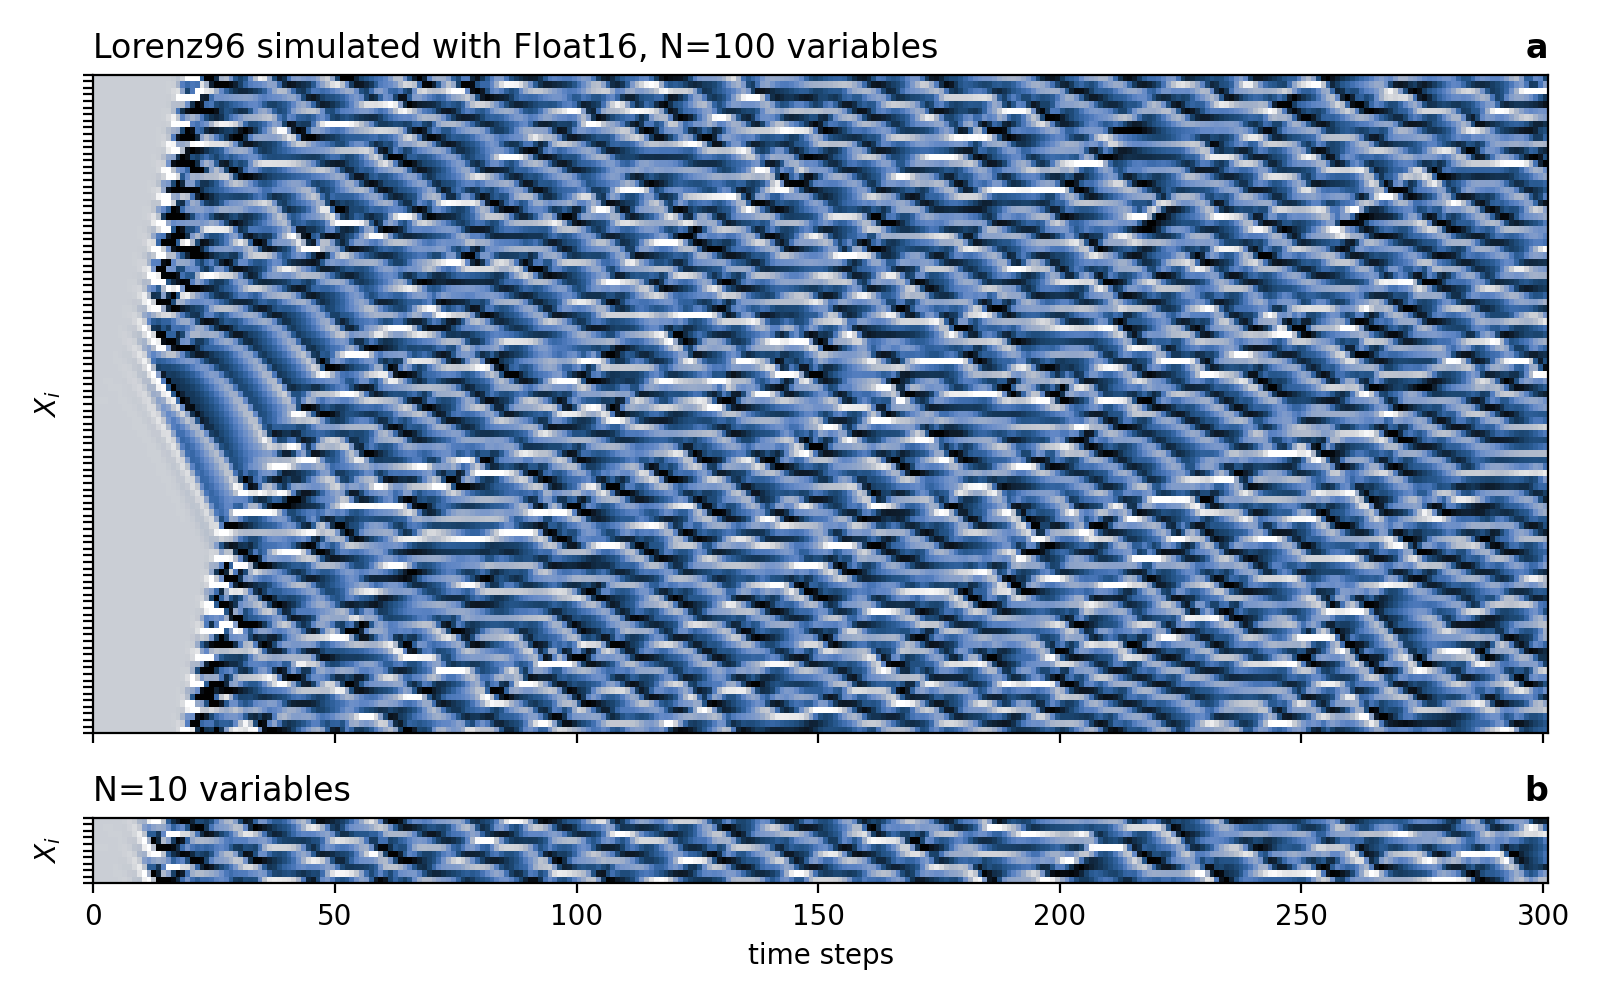
\includegraphics[width=1\textwidth]{Figs/hovmoeller.png}
%\caption{Solution of the Lorenz 1996 model presented as Hovmoeller diagram. (a) Float64 arithmetic, (b) Posit(16,1) arithmetic.}
%\label{fig:L96_hovmoeller}
%\end{figure}

A Hovmoeller diagram illustrates the chaotic dynamics simulated by the Lorenz 1996 model (Fig. \ref{fig:L96_hovmoeller}). The initial perturbation in $X_1$ is advected throughout the domain within the first time steps. After this first wake, the model's state becomes chaotic. Posit(16,1) represents well the dynamic, as shown in the comparison with Float64 for reference.

To quantify the forecast error, we run a set of 1000 forecasts per number format, starting from a random time step of a long control simulation. The simulation with Float64 is taken as reference truth. Float16 has an exponential error growth that starts much earlier than the error growth for Posit(16,1) (Fig. \ref{fig:L96_error}). Both formats have on average an identical error growth rate. Posits clearly cause a reduced rounding error compared to floats at all lead times, making posits a better suited number format for the simulation of the Lorenz 1996 model.

We now use the long control simulation with Float64 to produce a dataset that contains all prognostic variables as well as the arithmetic results of all intermediate terms calculated for the tendencies. 16-bit sonums are trained with this dataset, such that they can self-organize around the numbers that occur most frequently within the Lorenz 1996 model (Fig. \ref{fig:Sonum_decprec}b). Consequently, Sonum16 has a slightly higher decimal precision compared to posits for the mode of the data distribution. A second mode is created for the tendencies, for which numbers of the order of $10^{-1}$ frequently occur. The decimal precision of Sonum16 drastically drops beyond the largest numbers $O(100)$ in the Lorenz 1996 model, as no bitpatterns have to be used to encode these real numbers.

After training, the sonum circle (Fig. \ref{fig:sonum_circle}) is defined. All arithmetic operations are precomputed creating look-up tables for multiplication, addition and subtraction. No look-up table is created for division as the Lorenz 1996 equations (Eq. \ref{eq:L96s}) are written division-free ($s^{-1}$ is precomputed). We can now quantify the forecast error as for floats and posits, running a set of 1000 forecasts from the same initial conditions as used for floats and posits.

Sonum16 has a smaller forecast error compared to posits for the important lead times where the normalised RMSE exceeds 1\% (Fig. \ref{fig:L96_error}). Interestingly, although the error growth is much faster for the first time steps, it levels off afterwards and approaches the same error growth rate as for floats and posits once the normalised RMSE exceeds about 1\%. This points towards a higher potential of Sonum16, when the cause of the initial rapid error growth is understood and circumvented with adjustments in the training method. As discussed in the previous section, sonums can be trained to minimize the average decimal rounding error, an aspect that requires further analysis to understand the optimal distribution of decimal precision for a given application. Nevertheless, sonums already provide perspectives towards an optimal number format for a given application. The main characteristics presumably are: (i) high precision for the most frequently occurring numbers, (ii) a tapered precision towards the smallest numbers and (iii) no redundant bitpatterns for very large and very small numbers that do not occur. Posits fulfill these criteria better than floats, which is likely the reason why they outperform floats in the applications presented here.

%\begin{figure}
%\includegraphics[width=1\textwidth]{Figs/L96_error.pdf}
%\caption{Error growth in the Lorenz 1996 system as simulated with Float16, Posit(16,1) or Sonum16. The error has been normalised by the climatological forecast error. Shaded areas denote the interquartile range of 1000 forecasts with the respective format.}
%\label{fig:L96_error}
%\end{figure}


\section{Rounding modes}
\label{sec:rounding}

\subsection{Round to nearest}
\label{sec:roundnearest}

	\subsection{Stochastic rounding}
	\label{sec:stochastic_rounding} 

The default rounding mode for floats and posits is round-to-nearest tie-to-even. In this rounding mode an exact result $x$ is rounded
to the nearest representable number $x_i$. In case $x$ is half-way between two representable numbers, the result will be tied to the
even. A floating-point number $x_i$ is considered to be even, if its significand ends in a zero bit. These special cases are therefore
alternately round up or down, which removes a bias that otherwise persists (see Eq. \ref{eq:biased_rounding} for an example of biased rounding).
Let $x_1$ and $x_2$ be the closest two representable numbers to $x$ and $x_1 \leq x < x_2$ then
\begin{equation}
\op{round}_{\op{nearest}}(x) =
\begin{cases}
x_1 \quad &\op{if} x - x_1 < x_2 - x,  \\
x_1 &\op{if} x-x_1 = x_2 - x \op{~and~} x1 \op{~even}, \\
x_2 &\op{else}.
\end{cases}
\label{eq:roundnearest}
\end{equation}

For stochastic rounding, rounding of $x$ down to a representable number $x_1$ or up to $x_2$ occurs at probabilities that are proportional
to the distance between $x$ and $x_1$, $x_2$, respectively. Let $\delta$ be the distance between $x_1,x_2$, then

\begin{equation}
\op{round}_{\op{stoch}}(x) =
\begin{cases}
x_1 \quad &\op{with~probability}\quad 1 - \delta^{-1}(x - x_1)  \\
x_2 &\op{with~probability}\quad  \delta^{-1}(x - x_1).
\end{cases}
\label{eq:stochround}
\end{equation}

This behaviour is illustrated in Fig. \ref{fig:stochround}. In case that $x$ is already identical with a representable number no rounding is applied
and the chance to obtain another representable number is zero. For $x$ being half way between two representable numbers, the chance of
round up or round down is 50\%. The introduced absolute rounding error for stochastic rounding is always at least as big as for round-to-nearest,
and when low-probability round away from nearest occurs, it can be up to $\pm \delta$, whereas for round-to-nearest the error is bound by
$\pm \tfrac{\delta}{2}$. Although the average absolute rounding error is therefore larger for stochastic rounding, the expected rounding error
decreases towards zero for repeated roundings
\begin{equation}
\lim_{N\to \infty}\frac{1}{N} \sum_i^N \op{round}_{\op{stoch}}(x) = x
\end{equation}
as follows by inserting Eq. \ref{eq:stochround}. Stochastic rounding is therefore exact in expectation.

The stochastic rounding mode is implemented for Float16 and BFloat16. Software emulations of both number formats rely on conversion to Float32,
such that the exact result (to the precision provided by Float32) is known before conversion back to 16 bit. Instead of calculating the probabilities
given in Eq. \ref{eq:stochround}, we add a stochastic perturbation $\xi \in [-\tfrac{\delta}{2},\tfrac{\delta}{2}]$ to $x$ before round-to-nearest.
Let $r$ be uniformly distributed in $[0,1]$ then Eq. \ref{eq:stochround} can then be rewritten as

\begin{equation}
\op{round}_{\op{stoch}}(x) =
\begin{cases}
\op{round}_{\op{nearest}}(x +\tfrac{\delta}{2}(r - \tfrac{x-x_1}{\delta}) \quad & \op{if} x_1 = 2^n \op{~and~} x-x_1 < \tfrac{\delta}{4}  \\
\op{round}_{\op{nearest}}(x + \delta(r-\tfrac{1}{2})) & \op{else}.
\end{cases}
\end{equation}

The special case only occurs for $x$ being within $\tfrac{\delta}{4}$ larger than a floating-point number $x_1 = 2^n$, that means with zero significand.
In this case the distance from $x_1$ to the previous float is only $\tfrac{\delta}{2}$, which has to be accounted for.


\subsection{Efficient bitwise implementations}
\label{sec:bitwiseop}

\section{Error norms}
\label{sec:error_norms}

\subsection{Mean, absolute and relative error}
	
	\subsection{Decimal error and precision}
	\label{sec:decimal_precision}

The decimal precision is defined as \citep{Gustafson2017,Gustafson2017a}
\begin{equation}
\op{decimal} \op{precision} = -\log_{10} \vert \log_{10}( \frac{x_\text{repr}}{x_\text{exact}} ) \vert
\end{equation}
where $x_\text{exact}$ is the exact result of an arithmetic operation and $x_\text{repr}$ is the representable number
that $x_\text{exact}$ is rounded to, given a specified rounding mode. For the common round-to-nearest rounding mode,
the decimal precision approaches infinity when the exact result approaches the representable number and has a minimum
in between two representable numbers. This minimum defines the \emph{worst-case} decimal precision, i.e. the decimal
precision when the rounding error is maximised. The worst-case decimal precision is the number of decimal places that
are at least correct after rounding.

Fig. \ref{fig:decimal_precision} compares the worst-case decimal precision for various 16 and 8-bit floats and posits,
as well as 16-bit integers, the fixed-point format Q6.10 (6 integer bits, 10 fraction bits) and logarithmic fixed-point numbers
LogFixPoint16 and Approx14. Float16 has a nearly constant decimal precision of almost 4 decimal places, which decreases
for the subnormal numbers towards the smallest representable number $minpos$. 16-bit posits, on the other hand, show an
increased decimal precision for numbers around 1 and a wider dynamic range, in exchange for less precision for numbers
around $10^4$ as well as $10^{-4}$.  The machine precision $\epsilon$ (in analogy to the machine error, also known as
machine epsilon), defined as half the distance between 1 and the next representable number, is given in terms of decimal
precision and is summarised in Table \ref{tab:formats} for the various formats. Due to the no overflow/no underflow-rounding
mode, the decimal precision is slightly above zero outside the dynamic range.

The decimal precision of 16-bit integers is negative infinity for any number below 0.5 (round to 0) and maximised for the
largest representable integer $2^{15} - 1 =  32767$. Similar conclusions hold for the fixed-point format Q6.10, as the decimal
precision is shifted towards smaller numbers by a factor of $\tfrac{1}{2}$ for each additional fraction bit.

	\section{Type-flexibility through code composability}
	\subsection{A type-flexible programming paradigm}

Julia's programming paradigms of \emph{multiple-dispatch} and \emph{type-stability} facilitate the use of arbitrary number formats
without the need to rewrite an algorithm, while compiling functions for specific types \citep{Bezanson2017}. As this is an essential
feature of Julia and extensively made use of here, we briefly outline the benefits of Julia by computing the harmonic sum
$\sum_{i=1}^\infty \tfrac{1}{i}$ with various number types as an example. Analytically the harmonic sum diverges, but with
finite precision arithmetic several issues arise. With an increasing sum the precision is eventually lower than required to
represent the increment of the next summand. The integer i as well as its inverse $\tfrac{1}{i}$ have to be representable
in a given number format, and are also subject to rounding errors.

%\begin{figure}[htbp]
%\small
%\begin{minted}[breaklines,escapeinside=||,mathescape=true,baselinestretch=0.7, linenos, numbersep=3pt, bgcolor=mygray,gobble=2,
%frame=lines, fontsize=\small, framesep=2mm]{julia}
%function harmonic_sum(::Type{T},steps::Int=2000) where T
%
%    s = zero(T)
%    o = one(T)
%
%    for i in 1:steps
%
%        s_old = s
%        s += o/T(i)
%
%        if s == s_old    # check for convergence
%            println(Float64(s),i)
%            break
%        end
%    end
%end
%\end{minted}
%\caption{A type-flexible harmonic sum function in the Julia language.}
%\label{fig:harmsum}
%\end{figure}

Executing the function \texttt{harmonic\_sum} for the first time with a type \texttt{T} as the first argument, triggers Julia's
\emph{just-in-time} compiler (Fig. \ref{fig:harmsum}). The function is type-stable, as the types of all variables are declared
and therefore known to the compiler. At the same time Julia allows for type-flexibility, as its \emph{multiple-dispatch} means
that calling \texttt{harmonic\_sum} with another type \texttt{T2} will result in a separately compiled function for \texttt{T2}.
We can therefore compute the harmonic sum with arbitrary number types, as long as the zero-element \texttt{zero(T)};
the one-element \texttt{one(T)}; addition; division; conversion from integer and conversion to float are defined for \texttt{T}.

%\begin{figure}[htbp]
%\small
%\begin{minted}[breaklines,escapeinside=||,mathescape=true,baselinestretch=0.7, linenos, numbersep=3pt, bgcolor=mygray, gobble=2,
%frame=lines, fontsize=\small, framesep=2mm]{julia}
%julia> using SoftPosit
%julia> using BFloat16s
%julia> harmonic_sum(Float16)
%(7.0859375, 513)
%
%julia> harmonic_sum(BFloat16)
%(5.0625, 65)
%
%julia> harmonic_sum(Posit16)
%(7.77734375, 1024)
%\end{minted}
%\caption{Harmonic sum example use of the posit emulator \emph{SoftPosit.jl} in the Julia shell. \texttt{Posit16} is the Posit(16,1) standard.}
%\label{fig:harmsum2}
%\end{figure}

The harmonic sum converges after 513 elements when using Float16 (Fig. \ref{fig:harmsum2}). The precision of BFloat16
is so low that the sum already converges after 65 elements, as the addition of the next term $1/66$ is rounded back to
5.0625. We identify the addition of small terms to prognostic variables of size $\mathcal{O}(1)$ as one of the major challenges
with low precision arithmetic, which is discussed in more detail in section \ref{sec:mixed}. Using Posit(16,1), the sum only converges
after 1024 terms, due to the higher decimal precision of posits between 1 and 10.

\subsection{Analysis number formats}

\section{Information theory}
\label{sec:information}

\subsection{Entropy}
\label{sec:entropy}

\subsection{Mutual information}
\label{sec:mutual_information}

\subsection{Preserved information}
\label{sec:preserved_information}


